\documentclass[10pt]{article} % Font size - 10pt, 11pt or 12pt

\usepackage{amsmath}
\usepackage[hmargin=1.25cm, vmargin=1.5cm]{geometry} % Document margins

\usepackage[usenames,dvipsnames]{xcolor} % Allows the definition of hex colors

% Fonts and tweaks for XeLaTeX
\usepackage{fontspec,xltxtra,xunicode}
\defaultfontfeatures{Mapping=tex-text}
%\setmonofont[Scale=MatchLowercase]{Andale Mono}

% Colors for links, text and headings
\usepackage{hyperref}
\definecolor{linkcolor}{HTML}{506266} % Blue-gray color for links
\definecolor{shade}{HTML}{F5DD9D} % Peach color for the contact information box
\definecolor{text1}{HTML}{2b2b2b} % Main document font color, off-black
\definecolor{headings}{HTML}{701112} % Dark red color for headings
% Other color palettes: shade=B9D7D9 and linkcolor=A40000; shade=D4D7FE and linkcolor=FF0080

\hypersetup{colorlinks,breaklinks, urlcolor=linkcolor, linkcolor=linkcolor} % Set up links and colors

\usepackage{fancyhdr}
\pagestyle{fancy}
\fancyhf{}
% Headers and footers can be added with the \lhead{} \rhead{} \lfoot{} \rfoot{} commands
% Example footer:
%\rfoot{\color{headings} {\sffamily Last update: \today}. Typeset with Xe\LaTeX}

\renewcommand{\headrulewidth}{0pt} % Get rid of the default rule in the header
\renewcommand{\baselinestretch}{1.2}

\usepackage{titlesec} % Allows creating custom \section's

% Format of the section titles
\titleformat{\section}{\color{headings}
\scshape\Large\raggedright}{}{0em}{}[\color{black}\titlerule]

\title{Exploring Theory and Anisotropy Effects in Dendritic Phase-Field Model for Crystal Formation}
\author{Elliott Capek}

\begin{document}
\maketitle{}

\section{Variations on Model}
\subsection*{Zhao Model}
The Zhao model, described in [2], is most notable because of its use of noise to simulate thermal fluctuations in the crystal formation. The

\section{Anisotropy Effects}
\subsection*{Original Kanazawa Model}
The original model used in Kobayashi [1] introduces anisotropy by making interface layer thickness $\delta$ a function of $\theta$, the angle between $\nabla\phi$ and the x-axis. This dependence is given by:\\

\begin{equation*}
  \delta(\theta) = \delta_0(1 + \mu\cos(a_0(\theta-\theta_0)))
\end{equation*}

where $\delta_0$ is the average layer width, $\mu$ is the effect of anisotropy and $\theta_0$ is the rotation of the crystal. In Figure ($\ref{fig:r-delta-4}$) we show how $\delta$ varies with $\theta$ and the effect this has on the resultant crystal. Figures ($\ref{fig:r-delta-3}$) and ($\ref{fig:r-delta-6}$) show the same effect for anisotropies of $6$ and $3$, respectively.\\

These plots carry a lot of explanatory power. The lighter regions represent the lowest values of $\delta$. The system tends to minimize free energy, and $\delta$ makes a positive contribution to the value of $G$. We can think of $\delta(\theta)$ as a cost function that makes certain angles of $\nabla\phi$ more expensive than others. If we look at Figure ($\ref{fig-r-delta-4}$), the plot for $a=4$, we can see that 

\begin{figure}[h!]
  \centering
  \textbf{a. }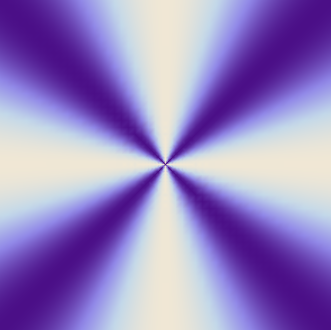
\includegraphics[width=0.2\textwidth]{../radial-anisotropy-4.png}
  \hspace{1cm}\textbf{b. }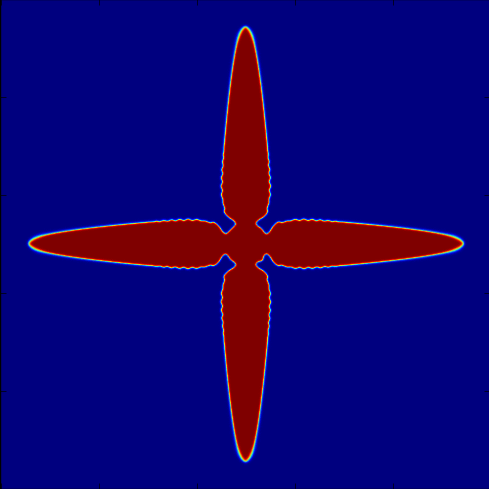
\includegraphics[width=0.2\textwidth]{../anis-4.png}
  \caption{\textbf{a.} Values of $\delta(\theta)$, where $\theta$ is the angular polar coordinate of points in the XY plane. Darker values correspond to larger values of $\delta$. \textbf{b.} The resulting crystal, plotted for the following parameters: $\a=4$,$dx=0.0003$, $F=1.8$ and $t=0.2$.}
  \label{fig:r-delta-4}
\end{figure}

\begin{figure}[h!]
  \centering
  \textbf{a. }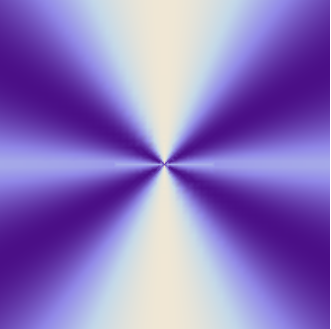
\includegraphics[width=0.2\textwidth]{../radial-anisotropy-3.png}
  \hspace{1cm}\textbf{b. }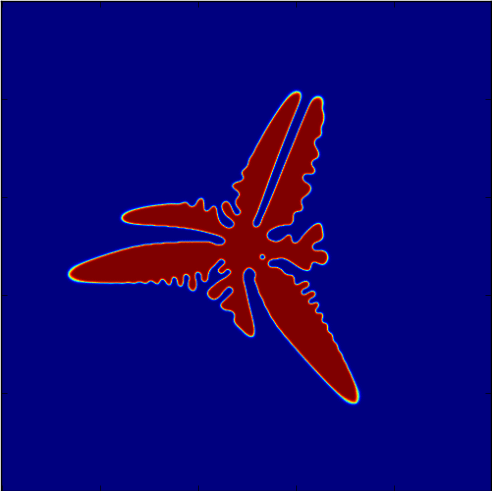
\includegraphics[width=0.2\textwidth]{../anis-3.png}
  \caption{$\delta$ and $\phi$, this time for $a=3$.}
  \label{fig:r-delta-3}
\end{figure}

\begin{figure}[h!]
  \centering
  \textbf{a. }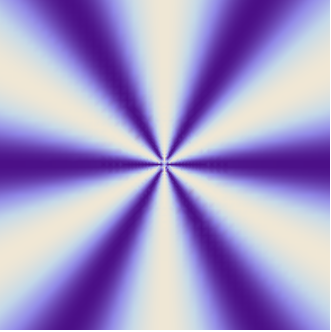
\includegraphics[width=0.2\textwidth]{../radial-anisotropy-6.png}
  \hspace{1cm}\textbf{b. }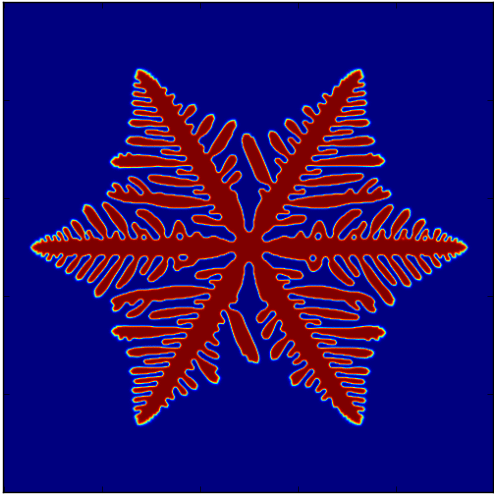
\includegraphics[width=0.2\textwidth]{../anis-6.png}
  \caption{$\delta$ and $\phi$, this time for $a=6$.}
  \label{fig:r-delta-6}
\end{figure}

\section{Reference}
\textbf{[1]} Kobayashi citation here\\

\end{document}
